\documentclass[oneside, a4paper, 12pt]{article}
\usepackage{thesis-style}
\usepackage{multirow}
\usepackage{amsmath,amsfonts,amssymb,amsthm,epsfig,epstopdf,titling,url,array}
\usepackage{mdframed}
\usepackage{tabularx, booktabs}
\usepackage{siunitx}
\usepackage{textcomp}

\sisetup{retain-explicit-plus}
\newcolumntype{L}[1]{>{\raggedright\arraybackslash}m{#1}}
\newcolumntype{C}[1]{>{\centering\arraybackslash}m{#1}}
\newcolumntype{Y}{>{\centering\arraybackslash}X}
\newcommand\TB{\rule[-1.5ex]{0ex}{4.7ex}} % "top&bottom" strut

\usepackage{listings}
\usepackage{color}

\usepackage{tcolorbox}
\usepackage[hidelinks]{hyperref}
\usepackage[inline]{enumitem}

\newcolumntype{Y}{>{\centering\arraybackslash}X}

\tcbuselibrary{theorems}

\theoremstyle{definition}
\newtheorem{definition}{Definíció}[section]
\newtheorem{assumption}{Feltétel}[section]
\newtheorem{stmt}{Állítás}[section]
\newtheorem{prof}{Bizonyítás}[section]

\newtcbtheorem[number within=section]{algorithm}{Algoritmus}%
{colback=green!5,colframe=green!35!black,fonttitle=\bfseries}{th}

\definecolor{mygreen}{rgb}{0,0.6,0}
\definecolor{mygray}{rgb}{0.5,0.5,0.5}
\definecolor{mymauve}{rgb}{0.58,0,0.82}
\definecolor{mygrayback}{rgb}{0.9,0.9,0.9}
\lstset{ %
backgroundcolor=\color{mygrayback},   % choose the background color; you 
%must
%add \usepackage{color} or \usepackage{xcolor}; should come as last argument
basicstyle=\small,        % the size of the fonts that are used for the code
breakatwhitespace=false,
breaklines=true, 
captionpos=b,
commentstyle=\color{mygreen},    % comment style
extendedchars=true,              % lets you use 
%frame=single,	                   % adds a frame 
keepspaces=true,                 % keeps spaces in 
keywordstyle=\color{blue},       % keyword style
language=C++,                 %
numbers=left,                    % where to put the line-numbers; possible
%values are (none, left, right)
numbersep=5pt,                   % how far the line-numbers are from the 
%code
numberstyle=\footnotesize\color{mygray}, % the style that is used for the
%line-numbers
rulecolor=\color{black},         % if not set, the frame-color may be 
%changed
%on line-breaks within not-black text (e.g. comments (green here))
showspaces=false,                % show spaces everywhere adding particular
%underscores; it overrides 'showstringspaces'
showstringspaces=false,          % underline spaces within strings only
showtabs=false,                  % show tabs within strings adding 
%particular
%underscores
stepnumber=1,                    % the step between two line-numbers. If 
%it's
%1, each line will be numbered
stringstyle=\color{mymauve},     % string literal style
tabsize=2,	                   % sets default tabsize to 2 spaces
title=\lstname                   % show the filename of files included with
%\lstinputlisting; also try caption instead of title
}



% Töltsd ki a saját szakdolgozatod adataival
\def\CIM{
Improved symbolic execution loop modeling for C like languages}
\def\SZERZO{Szécsi Péter}
\def\VEDESEVE{2018}

\def\TANSZEK{Programozási Nyelvek és Fordítóprogramok Tanszék}
\def\TEMAVEZETTO{Horváth Gábor}
\def\TEMAVEZETTOBEOSZTAS{Doktorandusz}
\def\TEMAVEZETO{Porkoláb Zoltán}
\def\TEMAVEZETOBEOSZTAS{Egyetemi docens}

\title{\CIM}
\author{\SZERZO}
\date{\VEDESEVE}	

\begin{document}
\pagestyle{empty}

% belső fedőlap
\begin{titlepage}

\begin{minipage}{0.40\linewidth}
\includegraphics[scale=0.3]{img/elte-cimer}
\end{minipage}
\begin{minipage}{0.50\linewidth}
\begin{center}
Eötvös Loránd University \\
Faculty of Informatics \\
\TANSZEK
\end{center}
\end{minipage}

\hrule
\vfill

\begin{center}
\Huge
\textbf{\CIM}
\normalsize
\end{center}

\vfill

\begin{minipage}[t]{0.5\linewidth}
\noindent
Supervisors:\\
\textbf{\TEMAVEZETO} \hfill \textbf{\TEMAVEZETTO}\\
\TEMAVEZETOBEOSZTAS  \hfill \TEMAVEZETTOBEOSZTAS
\end{minipage}
\begin{minipage}[t]{0.5\linewidth}
\begin{flushright}
Author: \\
\textbf{\SZERZO} \\
Computer Science MSc
\end{flushright}
\end{minipage}

\vfill

\begin{center}
\includegraphics[scale=0.1]{img/unkp}\\
\textit{\small{This study was supported by the \'UNKP-17-2 New National 
Excellence Program of the Hungarian Ministry of Human Capacities.}}


Budapest, \VEDESEVE
\end{center}

\end{titlepage}

\cleardoublepage

% tartalomjegyzék
\tableofcontents
\clearpage

\pagestyle{plain}
\setcounter{page}{4}


\section{Introduction}
During software development it is natural to make mistakes. Consequently,
writing various test cases is required in order to validate the behavior
of the program. In addition to the costs of test writing, it is possible that the developers fail
to cover all possible critical cases. Furthermore, test writing and running
often happens later than code development, but the costs of error correction
increases proportionally to elapsed time  \cite{fixcost}. This proves that 
testing alone is not necessarily sufficient to ensure code quality.  %Moreover,
%there are specific properties of a software - e.g. coding convention following 
%- which can not be checked by test cases.

The static analysis tools offer a different approach for code validation 
\cite{Zhivich2009} \cite{Bessey2010}, moreover, they can potentially check for 
some characteristics of the code -- which cannot be verified by testing -- e.g. 
the adherence to conventions.

These tools are given the source code as input, using which they build a model 
and make inferences based on that. The efficiency, accuracy, and runtime of the 
analysis changes depending on the complexity of the model.
The final output is a list of bug reports. However bugs are used quite 
liberally here; they do not necessarily imply program malfunctions, as 
optimisations or code convention nits are also included. Code chunks deemed 
fragile or to have potential portability problems are listed too, so there can 
be a wide variety of possible outputs.
This document focuses on static analysis primarily as a method of uncovering 
bugs.
 
Unfortunately, it is impossible to detect every 
bug only by using static analysis \cite{Rice:53}. Static analyzer tools might 
not be able to discover some bugs (these are called false negatives) or report 
correct code snippets as incorrect (false positives, see Fig \ref{fig:bes}). In 
the industry the goal of these tools is to keep the ratio of the false positive 
reports low while still be able to find real bugs.

\begin{figure}[!h]
	\begin{center}
		\begin{tabular}{ | l | c | r | }
			\hline
			& True error   & Non-error \\ \hline
			Reported error   & True Positive  & False Positive   \\ \hline
			No error report & False Negative & True Negative    \\
			\hline
		\end{tabular}
	\end{center}
	\caption{The different types of the static analysis results.}
	\label{fig:bes}
\end{figure}

Its important to note that another advantage of the static analyzer tools 
(against test cases) that the analysis happens without executing the source 
code, so it can be used without the running environment. Moreover, the code 
coverage of the analysis does not depends on the already written test case set 
and even can find bugs which is not covered by test cases e.g. unexpected 
corner cases on the input variables. 

The LLVM Clang Static Analyzer is a source code analysis tool which aims to 
find bugs in C,
C++, and Objective-C programs using - one of the most precise analysis methods 
- symbolic execution  \cite{King1975} \cite{Hampapuram2005}, i.e. it simulates 
the possible execution paths of the code. During symbolic execution, the 
program is being interpreted, on a function-by-function basis, without any 
knowledge about the runtime environment. It builds up and traverses an inner 
model of the execution paths, called \texttt{ExplodedGraph}, for each analyzed 
function. This method has exponential runtime and space complexity in the 
number of branches.


\section{The Clang Static Analyzer}

\emph{Clang} is an open-source compiler, which is based on the \emph{LLVM} 
project \cite{lattner:clang}. This is a quickly improving project, 
supported by various companies including e.g. Google, Apple, Samsung, Ericsson, 
etc. Moreover it is becoming more and more popular in the circle of compilers. 
Since Clang is built outstandingly modular, it is not simply a compiler but a 
complete framework for creating developer tools on C/C++/Objective-C 
languages. Its API is well documented and the software is well tested due to 
the wide user base.


The Clang Static Analyzer (CSA) -- as it is indicated by its name -- build 
around the Clang compiler. It is one of the most quickly developing open source 
static analysis tool. In this section the principles and the relevant 
implementation details of the CSA will be presented.
%%%
\subsection{Symbolic execution}
The CSA uses the symbolic execution static analysis algorithm which means it 
simulates the possible execution paths and tries make conclusions. It basically 
interprets the source code but instead of using the actual semantics, it 
defines an abstract one and models the state according to the defined one.

Unknown values is represented by symbols/symbolic values. The CSA makes 
constraints on these symbolic values during the analysis of the different 
paths. Among others, these constraints came from the condition on which a path 
may bifurcate. There is a constraint solver module in the analyzer which 
handles these and tries to deduce the conflicts (exclude the non-feasible 
paths). This is important since a bug found on a non-feasible path is 
considered as a false positive. The analysis stops if all of the execution 
paths are simulated and checked or it reaches a predefined limit.

The memory is represented by a hierarchic memory region system 
\cite{clang:memmodel}, the correspondence between symbolic values and memory 
regions is tracked. The state of a given program point contains this relation 
of bindings as well.

\begin{figure}[h]
	\centering
	\frame{\includegraphics[width=1\textwidth]{img/utvonalak}}
	\caption{The different execution paths of a simple function}
	\label{fig:exec_path}
\end{figure}

The analysis of the different execution paths can be done in any order, 
however, the evaluation of an expression (on a given path) must happen 
according to the language standard.  
During the simulation of the expressions the analyzer models the state of the 
program, means that one expression/instruction will create a transition between 
two states. A symbolic state can be viewed as a set of concrete program states, 
moreover, a simulated path is basically an analysis of these symbolic states in 
a well defined order. 

In order to be able to perform this process efficiently, the analyzer creates 
an inner model of the execution paths, called ExplodedGraph 
\cite{explodedgraph}. The nodes of the ExplodedGraph (called ExplodedNodes) are 
pairs, containing a symbolic program state and a program point. The program 
point determines the code location where the symbolic execution is in the 
source text. The directed edge between ExplodedNodes determines the sequencing.

Whenever the CSA encounters a branch in the symbolic execution, it creates new 
branches in the ExplodedGraph (see Fig \ref{fig:exploded_graph}). The paths
from the root to the leaves represents the analyzed paths. This means, that the 
number of leaves in the ExplodedGraph (and so the size of the graph) is 
exponential with respect to the branches in the execution. That results us a 
complex, precise but resource consuming method.

The ExplodedGraph is a simple directed acyclic graph. Whenever the analysis 
reachesan ExplodedNode which was already visited before, then the simulation 
will be stopped since the CSA would do the same (deterministic) reasoning what 
was already done. Note, that in case of concrete program states this would lead 
to an infinite loop, on the symbolic level this does not stand, since a
symbolic program state represents a set of real program states.

\begin{figure}[h]
	\centering
	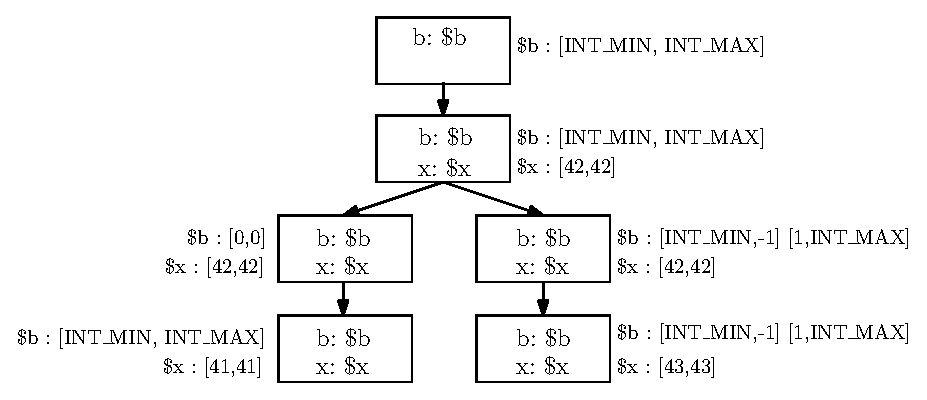
\includegraphics[width=1\textwidth]{img/explodedgraph.eps}
	\caption{The corresponding ExplodedGraph to the function presented on Fig 
		\ref{fig:exec_path}. The constraints made on the symbolic values are 
		shown next to the ExplodedNodes it belongs.}
	\label{fig:exploded_graph}
\end{figure}

In practice, the CSA constructs ExplodedNodes which does not represent any 
concrete transition between nodes but just help the simulation e.g. at some 
points the analyzer cleans up the stored but not necessary symbols and so it 
introduces a new node in order to smoothly fit this procedure into the flow of 
the analysis.

\begin{figure}[h]
	\centering
	\includegraphics[width=0.7\textwidth]{img/eg}
	\caption{A small part of the actual ExplodedGraph built by the Clang 
	Static Analyzer for the function shown on Fig \ref{fig:exec_path}.}
	\label{fig:exploded_graph2}
\end{figure}

According to the properties of the model, it can be declared, that the symbolic 
execution is a path sensitive algorithm, i.e. reaching any program state the 
CSA knows the whole path leading to the simulated point. Thereby the displaying 
of the bugs shows not only the location of the bug but the corresponding 
execution path as well. This productively helps the programmer to understand 
the problem more easily, even spending less time on fixing the bug.

\begin{figure}[h]
	\centering
	\includegraphics[width=1\textwidth]{img/view}
	\caption{A bug found by the Clang Static Analyzer can be represented in HTML format to make it more clear and understandable.}
	\label{fig:hibak_megjelenitese}
\end{figure}

\subsection{Implementation details}
\subsubsection{The process of the analysis}
The CSA works on a translation unit, analyzing its content function by function. So the the inner model is constructed for an analysis of a function and its states are represented in the ExplodedGraph.

Whenever -- during the simulation of a given path -- the CSA encounters a branch in the execution, it splits the states creating more children for the actually simulated ExplodedNode, and so constructs new paths to analyze. Moreover, the condition which caused the branching is stored and the assumption whether it is true or false as well. This can potentially results in restriction on the symbolic values, and so we collect information which help us on the upcoming decisions.

It is possible that the simulation encounters a call of an other function.
At this point the called function will be evaluated/analyzed on the spot of the call, knowing the calling context. This allows us to make a more precise analysis of the called function, since we potentially have information on the possible values of its arguments. The analysis of a function while knowing the calling context is called an \textit{inline} analysis. The other possibility -- when we have absolutely no information or precondition on the values of a function and it is analyzed so -- is called an \textit{top level} analysis. 

In order to decrease the rate of false positive reports and make the analysis more time efficient, the CSA will not reanalyze a function as top level if it was already analyzed as an inline function. The analyzer tries to inline as much function as possible. This is reached by creating the function call graph of the translation unit and the analysis order of the functions is determined by a post-traversal-walk TODO on this call graph.

As it was mentioned earlier, branches in the execution lead to an exponential number of \texttt{ExplodedNode}s.
This combinatorial explosion is handled in the Static Analyzer by restricting or even stopping
the analysis when given conditions are fulfilled. Terminating the analysis 
process may cause loss of potential true positive results, but it is 
indispensable for maintaining a reasonable resource consumption regarding the 
memory and CPU usage. 

These conditions are modeled by the concept of budget.
The budget is a collection of limitations on the shape of the \texttt{ExplodedGraph}.
These limitations include:
\begin{enumerate}  
	\item The maximum number of traversed nodes in the \texttt{ExplodedGraph}. 
	If 	this number is reached then the analysis of the simulated function stops.
	\item The size of the simulated call stack. When a function call is 
	reached then the analysis continues in its body as if it was inlined to the 
	place of call (interprocedural). There are several heuristics that may control 
	the	behavior of inlining process. For example the too large functions are 
	not	inlined at all, and the really short functions are not counted in the 
	size of	call stack.
	\item The number of times a function is inlined. The idea behind this
	constraint is that the more a function is analyzed, the less likely it 
	is that a 	bug will appear in it. If this number is reached then that 
	function will not be inlined again in this \texttt{ExplodedGraph}.
	\item The number of times a basic block is processed during the 
	analysis. This	constraint limits the number of loop iterations. When this 
	threshold is reached the currently analyzed execution path is aborted.
\end{enumerate}

The budget expression can be used in two ways. Sometimes it means the
collection of the limitations above, sometimes it refers to one of these
limitations. This will always be distinguishable from the context.

\subsubsection{The building process of the model}
The syntactic and semantic information of variables, functions and types
are required to perform the above described simulation.
A szimulációhoz szükséges a különböző változók, függvények, típusok 
szintaktikus és szemantikus tulajdonságainak ismerete.
Ezen információk a C/C++ forrásfájlok esetén a fordítás során is szükségesek.
A fordítók ezeket egy saját, jól struktúrált adatszerkezetben tárolják, egy 
absztrakt szintaxisfát építenek fel a kód elemzése során.
A gyakorlatban ez konkrét (adott platformra jellemző) információkat, illetve a 
szemantikus tulajdonságokat is tartalmazza.
Sőt, számos fordító esetében kör is előfordulhat benne. Ilyenkor csupán csak 
történeti okokból hívják az adott adatszerkezetet fának.
A felsorolt tulajdonságok alapján ez az adatszerkezet a szimbolikus végrehajtás 
számára nélkülözhetetlen információkat tartalmaz. 
Ebben rejlik a fő motivációja annak, hogy egy statikus elemző rendszert egy 
fordító köré építsünk,
amely képes az alapvetően szükséges információk strukturált előállítására. 
Fontos még, hogy az adatszerkezetben
tárolt információk helyessége jól tesztelt, hiszen minden fordítás során a 
kódgeneráláskor ugyanezek az
információk lesznek felhasználva. A CSA a Clang fordító által épített 
szintaxisfát használja.

Ezek után már elegendő információ áll rendelkezésre az elemző rendszer számára,
hogy (pár köztes lépésen keresztül) képes legyen felépíteni a szimulálás során 
létrejövő Exploded Graphot.

Az elemzés során használt modellt (az Exploded Graphot) a CSA egy
optimalizált \textit{mélységi bejárás} segítségével építi fel és járja be 
egyszerre.
Ennek fő oka, hogy a mélységi bejáráshoz elegendő csak az adott útvonalhoz
tartozó csúcsok memóriában tartása. Ezzel szemben egy szélességi bejárás során
az összes elemzett útvonalat a memóriában kell tartanunk az útvonalérzékenység
megtartása érdekében. Továbbá a mélységi bejárás esetén kevesebb kontextus 
váltásra van
szükség: az adott útvonal elemzése során kevés memóriarégió és szimbólum kerül
felhasználásra, nagyobb eséllyel találhatóak meg a felhasznált adatszerkezetek a
processzor gyorsítótárában, így hatékonyabban tudjuk végrehajtani az 
elemzést.

\begin{figure}[h]
	\centering
	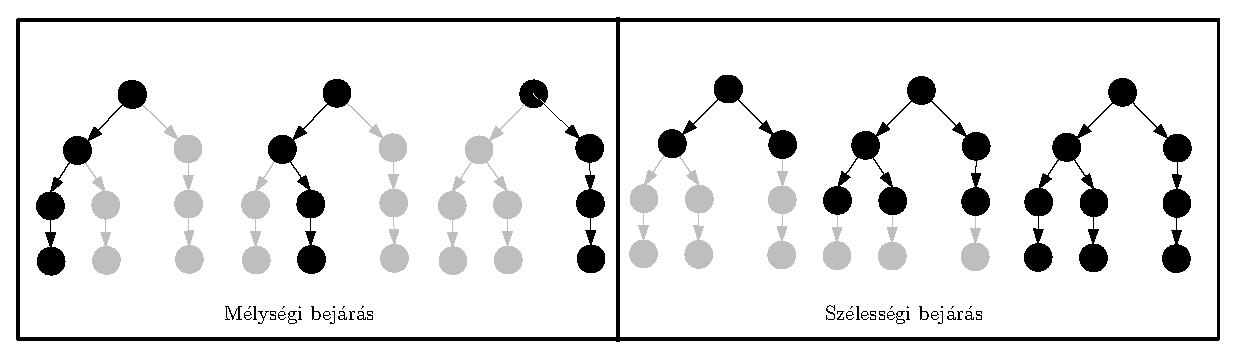
\includegraphics[width=1\textwidth]{img/memoria.eps}
	\caption{The different traverses of the Exploded Graph and the parts which 
	needs to be stored in the memory (black). Depth first search (left) and 
	breath first search (right).}
	\label{fig:bejaras_szemleltetes}
\end{figure}

Moreover, in order to use less memory during the analysis, the CSA clears the ExplodedNodes which are unnecessarily kept in the memory. This mainly means, the nodes that are created to help the analysis but not representing concrete state changes in the actual running of the program.

%%%%
An important technical note is that the building 
of the \texttt{ExplodedGraph} is based on the \texttt{Control Flow Graph} 
(\texttt{CFG}) of the functions. The \texttt{CFG} represents a source-level, 
intra-procedural control flow of a 
statement. This statement can potentially be an entire function body, or just a 
single expression. The \texttt{CFG} consists of \texttt{CFGBlocks} which are 
simply containers of statements. The \texttt{CFGBlocks}s essentially represent 
the basic blocks of the code but can contain some extra custom information. 
Although basic blocks and \texttt{CFGBlocks} are technically different, in the 
rest of the article the term basic blocks will be used for \texttt{CFGBlocks} 
as well for the sake of easier understanding and better illustration.

Thus during the analysis -- based on the function CFGs -- an 
\texttt{ExplodedGraph} is built up. A 
node of this graph (called \texttt{ExplodedNode}) contains a 
\texttt{ProgramPoint} (which determines the location) and a \texttt{State} 
(which contains any known information at that point). Its paths from the root 
to the leaves are modeling the different execution paths of the analyzed 
function. Whenever the execution encounters a branch, a corresponding branch 
will be created in the \texttt{ExplodedGraph} during the simulated 
interpretation.



\section{Motivation}
Currently, the analyzer handles loops quite simply. More precisely, it unrolls 
them 4 times by default and then cuts the analysis of the path where the loop 
would have been unrolled more than 4 times. This behavior is reached by the 
above presented basic block visiting budget (restriction no. 4).

Loss in code coverage is one of the problems with this approach to loop
modeling. Specifically, in cases where the loop is statically known to make 
more than 4 steps, the analyzer do not analyze the code following the loop. 
Thus, the naive loop handling (described above) could lead to entirely 
unchecked code.
Listing \ref{UnrollMot} shows a small example for that.

\lstset{language=C,caption={Since the loop condition is known at every 
		iteration, the analyzer will not check the 'rest of the function' 
		part in the 
		current state.},label=UnrollMot}
\begin{lstlisting}
void foo() {
  int arr[6];
  for (int i = 0; i < 6; i++) {
    arr[i] = i;
  }
  /*rest of the function*/
}\end{lstlisting}

According to the budget rule concerning the basic block visit number, the
analysis of the loop stops in the fourth iteration even if the loop 
condition is simple enough to see that unrolling the whole loop would not be 
too much extra work relatively. Running out of the budget implies (in this 
case) that the rest of the function body remains unanalyzed, which may lead to 
not finding potential bugs.
Another problem can be seen on Listing \ref{WidenMot}:
\lstset{language=C++,caption={The loop condition is unknown but the 
analyzer 
		will not generate a simulation path where n $\ge$ 4 (which can 
		result coverage 
		loss).},label=WidenMot}
\begin{lstlisting}
int num();
void foo() {
  int n = 0;
  for (int i = 0; i < num(); ++i) {
    ++n;
  }
  /*rest of the function, n < 4 */
}\end{lstlisting}

This code fragment results in an analysis which keeps track of the values of 
\texttt{n} and \texttt{i} variables (this information is stored in the State). 
In every iteration of the loop the values are updated accordingly. Note that 
updating the
State means that a new node is inserted into the \texttt{ExplodedGraph} with the 
new 
values. Since the body of the \texttt{num()} function is unknown, the 
analyzer can not find out its return value. Thus it is considered as 
unknown. This circumstance
makes the graph to split into two branches. The first one belongs to the symbolic
execution of the loop body assuming that the loop condition is true. The 
other one simulates the case where the condition is false and the execution 
continues after the loop. This process is done for every loop iteration, 
however, at the 4th time, assuming the condition is true, the path will be cut 
short according to the budget rule.
Even though the analyzer generates paths to simulate the code after the loop 
in the above described case, the value of variable \texttt{n} will be 
always less than 4 on these paths and the rest of the function will only be 
checked assuming this constraint. Since the analysis did not had any 
precondition on the possible values of the variables, this constraint not 
necessary correct. Most of the time this method results in coverage loss as 
well, since the analyzer will ignore the paths where n is more than 4.


\section{Proposed Solution}
%The current loop handling method in the Clang Static Analyzer is too 
%strict.
In this section two solutions are presented to resolve the above mentioned
limitations on symbolic execution of loops in the Clang Static Analyzer. It 
is important to note that these enhancements are incremental in the sense 
that the original method is brought back on examples which are too complex to handle at the moment. For the sake of simplicity a 
"division by zero" will illustrate the bug we intend to find in the following examples.

\subsection{Loop Unrolling Heuristics}
Loop unrolling means we have identified heuristics and patterns (such as 
loops
with small number of branches and small known static bound) in order to find
specific loops which are worth to be completely unrolled. This idea is 
inspired by the following example:

\lstset{language=C++,caption={Complete unrolling of the loop makes it possible 
to find the division by zero error.},label=UnrollEx}
\begin{lstlisting}
void foo() {
  for (int i = 0; i < 6; i++) {
    /*simple loop which does not
    change 'i' or split the state*/
  }
  int k = 0;
  int l = 2/k; // Division by zero
}\end{lstlisting}

In the current solution a loop has to fulfill the following conditions in order 
to be unrolled:
\begin{enumerate}  
	\item The loop condition should arithmetically compare a variable -- 
	which is known at the beginning of the loop -- to a literal (like: 				\texttt{i~<~6} or \texttt{6~$\ge$~i})
	\item The loop should change the loop variable only once in its body 
	and the	difference needs to be constant. (This way the maximum number of 
	steps can be estimated.)
    \item There is no alias created to the loop variable.
	\item The estimated number of steps should be less than 128. (Simulating 
	loops which takes thousands of steps because they could single handedly 
	exhaust the budget.)
	\item The loop must not generate new branches or use \texttt{goto} 
	statements.
\end{enumerate}

By using this method, the bug on the Listing \ref{UnrollEx} example can be 
found successfully.

\subsection{Loop Widening}
The final aim of widening is quite the same as the unrolling, to increase 
the coverage of the analysis. However, it reaches it in a very different way. 
During widening the analyzer simulates the execution of an arbitrary number 
of iterations. The analyzer already has a widening algorithm which reaches 
this behavior by discarding all of the known information before the last step 
of the loop. So the analyzer creates the paths for the first 3 steps and 
simulate them as usual, but in order to avoid losing the first precise simulation branches, the widening (means the invalidating) happens 
before the 4th step. 
This way the coverage will be increased, however, this method is disabled by 
default, since it can easily result in too much false positives. Consider the 
example on Listing \ref{WidenProb}.
\\

\lstset{language=C++,caption={Invalidating every known information (even 
those which are not modified by the loop) can easily result in false 	
positives.},label=WidenProb}
\begin{lstlisting}
int num();
void foo() {
  bool b = true;
  for (int i = 0; i < num(); ++i) {
    /*does not changes 'b'*/
  }
  int n = 0;
  if (b)
    n++;
  n = 1/n; // False positive:
           // Division by zero
}\end{lstlisting}
In this case the analyzer will create and check that unfeasible path where 
the variable \texttt{b} is false, so \texttt{n} is not incremented and lead 
into a division by zero error. Since this execution path would never be 
performed while running the analyzed program, it is considered a false positive. My aim 
was to give a more precise approach for widening. There was already conversation within the community about some possible enhancements \cite{Widening}.

One of the main principles is that the analysis should still continue after the block 
visiting budget is exhausted and the information of only those variables should be invalidated which are possibly modified by the loop, e.g. a statement, like \texttt{arr[i] = i} where \texttt{i} is the loop variable, means that we discard the data on the whole \texttt{arr} array but nothing else).
For this I developed a solution which checks every possible way in which a 
variable can be modified in the loop. Then these cases are evaluated and if it 
encounters a modified variable which cannot be handled by the invalidation 
process (e.g.: a pointer variable), then the loop will not be widened and we
return to the conservative method. This mechanism ensures that we do not create 
nodes that contain invalid states.
This approach helps us to cover cases and find bugs like the one illustrated on 
Listing \ref{WidenEx} without reporting false positives  
presented on Listing \ref{WidenProb}.

\lstset{language=C++,caption={Invalidating the information on only the possible 
changed variables can result higher coverage (while limiting the number of the 
found false positives).}, label=WidenEx}
\begin{lstlisting}
int num();
void foo() {
  int n = 0;
  for (int i = 0; i < num(); ++i) {
    ++n;
  }
  if (n > 4) {
    int k = 0;
    k = 1/k;  // Division by zero error
  }
}\end{lstlisting}

The bug is found by invalidating the known information on variable
\texttt{n} (and \texttt{i} as well). This makes the analyzer to create a 
branch
where it checks the body of the \texttt{if} statement and finds the bug.
However, this solution has its own limitations when dealing with nested 
loops. 
Consider the case on Listing \ref{WidenEx2}.
\lstset{language=C++,caption={The naive widening method does not handle 
well the nested loops. In this example the outer loop will not be widened.},label=WidenEx2}
\begin{lstlisting}
int num();
void foo() {
  int n = 0;
  for (int i = 0; i < num(); ++i) {
    ++n;
    for (int j = 0; j < 4; ++j) {
      /*body that does not change n*/
    }
  }
  /*rest of the function, n <= 1 */
}\end{lstlisting}

In this scenario, when the analyzer first step into the outer loop (so it assumes
that \texttt{i < num()} is true) and encounter the inner loop, it consumes
its (own) block visiting budget. (This implies that it will be widened, although
in this case it means that only the inner loop counter (\texttt{j}) information
is discarded.) After moving on to the next iteration, we may assume that we
are on the path where the outer loop condition is true again. Due to the fact that the budget was already exhausted in the previous iteration, the next visit of the first
basic block of the inner loop (the condition) means that this path will be
completely cut off and not analyzed. This results in the outer loop not reaching the step number where it would been widened. Furthermore, the outer loop
will not even reach the 3rd step, even the 2nd is stopped at in its body
(as described above). This causes the problem that even though the 
loop widening method is used, the rest of the function will be analyzed by the 
assumption \texttt{n <= 1}.

In order to deal with the above described nested loop problem, I have 
implemented a replay mechanism. This means that whenever we encounter an inner 
loop which already consumed its budget, we replay the analysis process of the 
current step of the outer loop after performing a widening first. This ensures
the creation of a path which assumes that the condition is false and simulates 
the execution after the loop while the possibly changed information are 
discarded. This way the analyzer will not exclude some feasible path 
because of the simple loop handling which solves the problem.

An additional note to the widening process is that it makes sense to analyze the branch 
where the condition is true with the widened State as well. The example on 
Listing \ref{WidenNested} shows a case where this is useful.
\\
\\
\lstset{language=C++,caption={The replay mechanism successfully helps us to 
		find the possible error the outer loop.},label=WidenNested}
\begin{lstlisting}
int num();
void foo() {
  int n = 0;
  int i;
  for (i = 0; i < num(); ++i) {
    if (i == 7) {
      break;
    }
    for (int j = 0; j < 4; ++j) {/* */}
  }
  int n = 1 / (7 - k);
         // ^ Possible division by zero
}\end{lstlisting}
This way the analyzer will produce a path where the value of \texttt{i} is 
known
to be 7, so it will be able find the possible division by zero error.
	
\subsection{Infrastructure improvements}\label{sec:inf}
The discussed approaches heavily rely on the fact that we are able to 
perform the following actions:
\begin{enumerate}
	\item Decide on any \texttt{ExplodedNode} whether it simulates a body of a 
	loop or not,
	\item Recognize the entering and exiting point of a loop on the simulated 
	path.
\end{enumerate}

However, this information was not provided by the analyzer earlier. Considering the 
lexical nature of the loops, their entrance and exit points can unambiguously 
fit into the \texttt{CFG}. 

The \texttt{ProgramPoint} provides the \texttt{LocationContext} which implements a stack data structure for having the information on the different locations of the code.  This implies that the callstack can be represented via this structure in a straightforward manner (and is contained by the \texttt{LocationContext}).
Since storing the currently simulated loops fits into a stack data structure as well, this information -- called \texttt{LoopContext} -- understandably was implemented as the part of the \texttt{LocationContext} too instead of having them in the \texttt{Store}. Both the \texttt{Store} and the \texttt{LocationContext} are part of an \texttt{ExplodedNode} in form of a pointer. However, these structures use copy-on-write semantics, and the \texttt{LocationContext} changes way less times, this decision saves us memory. 

\section{Evaluation}

The effect of the described loop modeling approaches was measured on various 
C/C++ open source projects. These are listed on Table \ref{tab:lines}.

\begin{table}[!htb]
	\centering
\begin{tabular}{ |c||c|c| }
	\hline
	Project & LoC & Language \\
	\hline
	TinyXML & 20k & C++ \\
	\hline
	Curl & 21k & C  \\ 
	\hline
	Redis & 40k & C \\ 
	\hline
	Xerces & 228k & C++ \\ 
	\hline
	Vim & 540k & C \\ 
	\hline
	OpenSSL & 550k & C  \\ 
	\hline
	PostgreSQL & 950k & C \\ 
	\hline
	FFmpeg & 1080k & C \\	
	\hline
\end{tabular}
\caption{The projects used for profiling, their length in code lines, and 
language.}\label{tab:lines}
\end{table}

\subsection{Coverage and the number of explored paths}
Keeping track of these statisics are already part of the analyzer. The 
coverage percentage is based on the ratio of the visited and the total number 
of basic blocks in the analyzed functions (instead of the number of visited statements),
which results in a small imprecision. 
It is important to note that the introduced loop modeling methods require having 
additional loop entrance and exit point information (described in section 
\ref{sec:inf}) in the \texttt{CFG}. This can lead to having more 
basic blocks in the \texttt{CFG} and it can affect the statistics. As a result, 
even statistics produced by using the current loop modeling 
approach were measured with this information added to the \texttt{CFG}.

The coverage and the number of explored paths are generated for every 
translation unit and then summarized. This means that header files which 
are included in more than one translation unit can influence more statistics.
However, by using this summarization process consistently for every measurement 
the results reflect the reality. 

The tables presented in this section summarize measurement results using 
different loop modeling approaches: the current practice (denoted by Normal)
and the hereby introduced loop unrolling (Unroll) and loop widening (Widen)
methods separately and simultaneously (U+W).

\begin{table}[!htb]
	\centering
\begin{tabular}{ |c||c|c|c|c| } 
	\hline
	Project & Normal & Unroll & Widen & U + W \\
	\hline \hline
	TinyXML & 84.2 & 84.2 & 85.1 & 85.1 \\ 
	\hline
	Curl & 76.2 & 76.9 & 77.7 & 77.2 \\ 
	\hline
	Redis & 68.5 & 69.1 & 68.5 & 71.3 \\ 
	\hline
	Xerces & 92.3 & 92.4 & 92.7 & 92.7 \\ 
	\hline
	Vim & 60.4 & 60.6 &	60.6 & 60.7 \\ 
	\hline
	OpenSSL & 97.4 & 97.5 & 97.7 & 97.7 \\ 
	\hline
	PostgreSQL & 76.9 &	77.0 & 76.9 & 76.9 \\ 
	\hline
	FFmpeg & 86.1 & 86.3 & 87.0 & 86.8 \\	
	\hline
\end{tabular}
\caption{The code coverage of the analysis on the evaluated projects expressed 
in percentage.}\label{tab:cov}
\end{table}

Table \ref{tab:cov} shows the coverage difference using the introduced 
approaches. On most of the projects, analysis coverage was strictly increased by
using any of the proposed approaches. The widening method had a stronger 
influence on the coverage in the average case. However, the complete unroll of 
specific loops could result in a higher coverage as well (e.g. Curl, Redis).
In general, enabling both of them was the most beneficial with respect to the 
coverage.

\begin{table}[!htb]
	\centering
\begin{tabular}{ |c||r|r|r|r| } 
	\hline
	Project & Normal & Unroll & Widen & U + W \\
	\hline \hline
	TinyXML & 14\,452 & 15\,460 & 14\,765 & 15\,773 \\ 
	\hline
	Curl & 18\,272 & 18\,577 & 28\,835 & 24\,279 \\
	\hline
	Redis & 69\,857 & 70\,097 & 98\,446 & 100\,929 \\ 
	\hline
	Xerces & 395\,615 & 398\,077 & 430\,989 & 433\,358 \\ 
	\hline
	Vim & 155\,451 & 157\,266 & 188\,136 & 173\,121 \\ 
	\hline
	OpenSSL & 687\,175 & 687\,932 & 700\,464 & 701\,013 \\ 
	\hline
	PostgreSQL & 382\,660 & 383\,874 & 453\,188 & 419\,118  \\ 
	\hline
	FFmpeg & 466\,613 & 458\,480 & 571\,399 & 521\,725  \\ 		
	\hline
\end{tabular}
\caption{The numbers of explored execution paths using different loop modeling
approaches.}\label{tab:pathnum}
\end{table}
Table \ref{tab:pathnum} presents the numbers of analyzed execution paths.
As expected, both introduced loop modeling methods resulted in a higher number of
simulated paths on (almost) all of the projects. The only exception is the unrolling 
approach on the FFmpeg project, which caused the budget limiting the number of 
traversed \texttt{ExplodedNode}s to exhaust earlier, slightly decreasing 
the number of checked paths. Enabling both of the features resulted in similar or 
fewer number of explored paths than the runs using only widening. 
This effect can be explained in two ways:   
\begin{enumerate*} [label={(\arabic*)}, noitemsep]
	\item the analyzer prefers to completely unroll loops rather than widen them, 
    which results in a more precise modeling of the state and can exclude unfeasible 
    paths,
	\item the simultaneous use of the methods can lead to exhausting the budget on earlier paths, where the analysis will be terminated.
\end{enumerate*}

\subsection{Found bugs}
\begin{table}[!htb]
	\centering
\begin{tabular}{ |c||c|c|c|c| } 
	\hline
	Project & Normal & Unroll & Widen & U + W \\
	\hline \hline
	TinyXML & 1 & 1 & 3 & 3 (+200\%) \\
	\hline
	Curl & 16 & 16 & 16 & 16 (0\%) \\ 
	\hline
	Redis & 55 & 58 & 55 & 59 (+7.27\%) \\ 
	\hline
	Xerces & 62 & 62 & 61 & 61 (-1.61\%) \\ 
	\hline
	Vim & 74 & 74 & 76 & 78 (+5.4\%) \\
	\hline
	OpenSSL & 152 & 152 & 153 & 153 (+0.66\%) \\ 
	\hline
	PostgreSQL & 323 & 323 & 327 & 331 (+2.48\%) \\ 
	\hline
	FFmpeg & 425 & 420 & 423 & 454 (+6.82\%) \\ 		
	\hline
\end{tabular}
\caption{The number of bug reports produced by the analyzer.} \label{tab:reportnum}
\end{table}
The number of bug reports using the different loop modeling methods can be seen
in Table \ref{tab:reportnum}. The increase in analysis coverage and in the number of 
checked paths usually implies an increased number of found bugs, which indeed can be 
observed on the numbers. However, it is important to note that the upsurge of the number 
of explored execution paths described in Table \ref{tab:pathnum} considerably outweighs 
the moderate rise in the number of bug reports.
Since the loop widening method creates more new paths by discarding informations on the values of variables, it could introduce the risk of analyzing paths that lead to false positives.
However, from the results it seems that this was not a problem in practice: relative to the increase in the number of analyzed paths, the number of reports hardly increased. Moreover, based on studying the environment of the found bugs, the ratio of false positive findings was low (beside some clear true positive) among the newly detected bugs.

\subsection{Analysis time}

\begin{table}[!htb]
	\centering
\begin{tabular}{ |c||c|c|c|c| } 
	\hline
	Project & Normal & Unroll & Widen & U + W \\
	\hline \hline
	TinyXML & 0:51 & 0:51 & 0:52 & 0:52 (+2\%) \\ 
	\hline
	Curl & 0:50 & 1:06 & 0:55 & 1:05 (+30\%) \\ 
	\hline
	Redis & 2:06 & 2:11 & 2:28 & 2:10 (+3\%) \\ 
	\hline
	Xerces & 3:38 & 3:34 & 3:37 & 3:39 (+0.5\%) \\ 
	\hline
	Vim & 3:11 & 3:26 & 3:18 & 3:27 (+3\%) \\
	\hline
	OpenSSL & 2:04 & 2:22 & 2:13 & 2:19 (+8.3\%) \\
	\hline
	PostgreSQL & 7:03 & 8:32 & 7:48 & 7:59 (+13\%) \\
	\hline
	FFmpeg & 9:40 & 10:22 & 10:14 & 11:20 (+17\%) \\
	\hline
\end{tabular}
\caption{Average measured time of the analysis expressed in minutes. 
(Average of 5 runs.)}\label{tab:time}
\end{table} 
The running time on different projects is showed in Table \ref{tab:time}.
Although the widening method lead into more analyzed execution paths, the analysis time increase was more intense after enabling the unrolling process. This is possible due to the fact that unrolling leads to long paths where the \texttt{State} usually contains more information (constraints on variable values), which is very expensive in respect of running time. 
In general there was only a minor increase in the analysis time at all examined projects which suggests a good scalability of the proposed improvements.


\section{Future work}
The heuristic patterns for completely unrolled loops could be extended to 
involve loops whose bound is a known variable which is not changed in the body. 
Furthermore, even more general rules would be beneficial: consider loops where  
the value variables are known at the beginning and they are affected by a known 
constant change by every iteration. These improvements have not been implemented
yet due to some technical and framework limitations.

During the widening process we invalidate any possibly changed information. 
However, a change made on a pointer could mean that we need to 
invalidate all variables due to the lack of advanced pointer analysis. Therefore, 
introducing pointer analysis algorithms to the analyzer could help to develop a 
more precise invalidation process.

The infrastructural improvements enable the analyzer to provide entry points 
for bug finding modules (checkers) on loop entrances/exits and identify the 
currently simulated loop for every \texttt{ExplodedNode}. On top of these entry 
points new checkers can be implemented e.g. a check for finding possible 
infinite loops.


\section{Conclusion}

Two alternative approaches was introduced for improving the simulation of loops during symbolic 
execution. These were implemented and subsequently evaluated on various open 
source projects, with a clear improvement of code coverage in general. The new methods make it possible to explore previously skipped, feasible execution paths, especially when both of them are used in conjunction.

The required changes done to the underlying infrastructure should also ease the 
implementation of future enhancements. In particular, information tracked by the 
analysis about location contexts were expanded with additional fields.
While code coverage was measured to have increased by an average of 0.8\% and the 
number of explored execution paths by an average of 16\%, there 
was a noticeable performance penalty as well. A general increase in the runtime was observed, with an average of 9.5\% . The number of simulated paths also increased proportionally with the time taken, suggesting this time was well 
spent. In conclusion, if the user does not mind taking $\sim$10\% more time
for a more comprehensive analysis, then it is beneficial to enable the proposed
feature set by default. 
\section{Acknowledgement}
I would like to thank Laszlo Makk and the members of the \texttt{CodeChecker} 
team at Ericsson for their valuable and helpful suggestions on the paper. 

This study was supported by the \'UNKP-17-2 New National Excellence Program of 
the Hungarian Ministry of Human Capacities.
\begin{center}
	\includegraphics[scale=0.2]{img/unkp}\\
\end{center}

% tartalom

% 2012 ACM Computing Classification System (CSS) concepts
% Generate at 'http://dl.acm.org/ccs/ccs.cfm'.

% \ccsdesc[500]{Software and its engineering~General programming languages}
% \ccsdesc[300]{Theory of computation~Program analysis}
% end generated code

% Legacy 1998 ACM Computing Classification System categories are also
% supported, but not recommended.
%\category{CR-number}{subcategory}{third-level}[fourth-level]
%\category{D.3.0}{Programming Languages}{General}
%\category{F.3.2}{Logics and Meanings of Programs}{Semantics of Programming
%Languages}[Program analysis]





% The 'abbrvnat' bibliography style is recommended.

%\bibliographystyle{abbrvnat}

\bibliographystyle{apalike}
\bibliography{loopbibliography}

\end{document}
